\documentclass[%
  fontsize=11pt,%
  paper=a4,%
  headinclude=false,%
  foodinclude=false,%
  DIV=16%
]{scrartcl}

%%%%%%%%%%%%%%%%%%%%%%%%%%%%%%%%%%%%%%%%%%%

\usepackage{etex}
\usepackage[komastyle]{scrpage2}
\usepackage[greek,english]{babel}
\usepackage[utf8x]{inputenc}
\usepackage{amssymb,amsmath,amsfonts}
\usepackage{enumerate, enumitem}
\usepackage{wrapfig,enumitem,tabularx,hyperref}
\usepackage[all]{tcolorbox}

% Frame around page
\usepackage{tikz}
\usetikzlibrary{calc,shapes}
\usetikzlibrary{decorations.pathmorphing}

% Maybe unnecessary
\usepackage[detect-weight=true, detect-family=true]{siunitx}
\DeclareSIUnit\point{pt}

% Tcolorbox and minted configuration
\setminted[latex]{autogobble,fontsize=\scriptsize,linenos=false,breaklines}

\tcbset{%
  fonttitle=\bfseries,
  size=fbox,
  boxsep=2.0pt,
  arc=1mm,
  colback=white,
  colframe=red!75!black}

\newtcbinputlisting[]{\codeFromFile}[6][]{%
  listing engine=minted,
  minted options={#1},
  minted language=#2,
  listing file={#3},
  title={\scriptsize\centering #4},
  label=#5,
  listing only,
  breakable,
  #6
}

%%%%%%%%%%%%%%%%%%%%%%%%%%%%%%%%%%%%%%%%%%%

% Redefine footnotes. Maybe unnecessary
\makeatletter
\renewcommand{\@makefnmark}{\makebox{\normalfont[\@thefnmark]}}
\makeatother

% Custom smaller \maketitle
\makeatletter
\renewcommand{\maketitle}{
  \begin{center}
    \usekomafont{title}{\huge \@title\par}
    \vskip 1em
    \usekomafont{title}{\@subtitle}
  \end{center}
  \par
  \vskip 2em
  }
\makeatother

% Background frame
\newcommand{\backgroundframe}{
  \begin{tikzpicture}[overlay,remember picture]
    \draw [line width=1pt]
      %,segment length=<length>,amplitude=<length>
      ($ (current page.north west) + (1cm,-1cm) $)
      rectangle
      ($ (current page.south east) + (-1cm,1cm) $);
  \end{tikzpicture}
  }



\title{\LaTeX Fundamentals}
\subtitle{The Very Basics}
\date{}

\begin{document}

\pagestyle{empty}
\backgroundframe
\maketitle
%
% \codeFromFile([minted settings]){language}{file}{Title}{label}{additional tcolorbox settings}
\par\begin{wrapfigure}{R}[1.5cm]{5.5cm}
  %
  \centering
  %
  % Installation
  %
  \begin{tcolorbox}[size=fbox,title={\centering\scriptsize Installation},before upper=\scriptsize]
    \begin{tabularx}{\linewidth}{lX}
      Linux & \ttfamily apt-get install texlive-full\\
      MacOS & See \url{goo.gl/UMzDfV}\\
      Windows & See \url{goo.gl/Z19eiz}
    \end{tabularx}
  \end{tcolorbox}
  %
  % Mare Minimum Setup
  %
  \codeFromFile{latex}{material/minimal.tex}{Bare Minimum}{minimal}{}
  %
  % Minimal Working Example
  %
  \codeFromFile{latex}{material/mwe.tex}{\href{https://en.wikipedia.org/wiki/Minimal_Working_Example}{Minimum Working Example}}{mwe}{listing and comment, comment={\scriptsize Compilation:\\\texttt{pdflatex yourdocument.tex}}}
  %
  % Classes
  %
  \begin{tcolorbox}[size=fbox,title={\centering\scriptsize\ttfamily Classes},before upper=\scriptsize]
    \begin{tabularx}{\linewidth}{>{\ttfamily}lX}
      scrartcl & Small documents, short articles/reports\\
      scrreprt &  Longer reports, seminar papers, smaller theses\\
      scrbook  & Long works like books or dissertations\\
      scrlttr2 &  Letters
    \end{tabularx}
  \end{tcolorbox}
  %
  % Important Options
  %
  \begin{tcolorbox}[size=fbox,title={\centering\scriptsize Important \texttt{Options}},before upper=\scriptsize]
    \begin{tabularx}{\linewidth}{lX}
      \texttt{paper}& \ttfamily a4, a5, letter, \ldots\\
      \texttt{BOCR}& \ttfamily Longer reports, seminar papers, smaller theses\\
      \texttt{DIV}& \ttfamily Long works like books or dissertations\\
      \texttt{fontsize}& \ttfamily 8pt, 9pt, 10pt, \ldots
    \end{tabularx}
  \end{tcolorbox}
\end{wrapfigure}

%
\LaTeX{} -- short for Lamport-\TeX{}, originated from Leslie Lamport -- is the approach to create a more user-friendly and modern way to interact with the typesetting program \TeX{} of Donald Knuth (abr. for \textgreek{Τέχνη}, \textit{art, craft}).
%
The key ideas of \LaTeX{} to take away are:
%
\begin{itemize}
  \item Differentiate between the \textit{content} and the \textit{layout}: The former is written in a plain text editor of choice and is then \textit{given} to the professional typesetter \TeX{}.
  \item Forget your MS Word habits: \LaTeX{} is capable of everything but the more you force it into special solutions, the more pitfalls will arise!
\end{itemize}

\section*{Configurations}
%
Configurations
Usually blank line, in special environments (e.g. tables) \textbackslash\textbackslash \ldots

\section*{Important Packages}

test



%\noindent\begin{minipage}{0.5\textwidth}
%\inputminted{latex}{example.tex}
%\end{minipage}
%\hfill
%\begin{minipage}{0.5\textwidth}
%  \frame{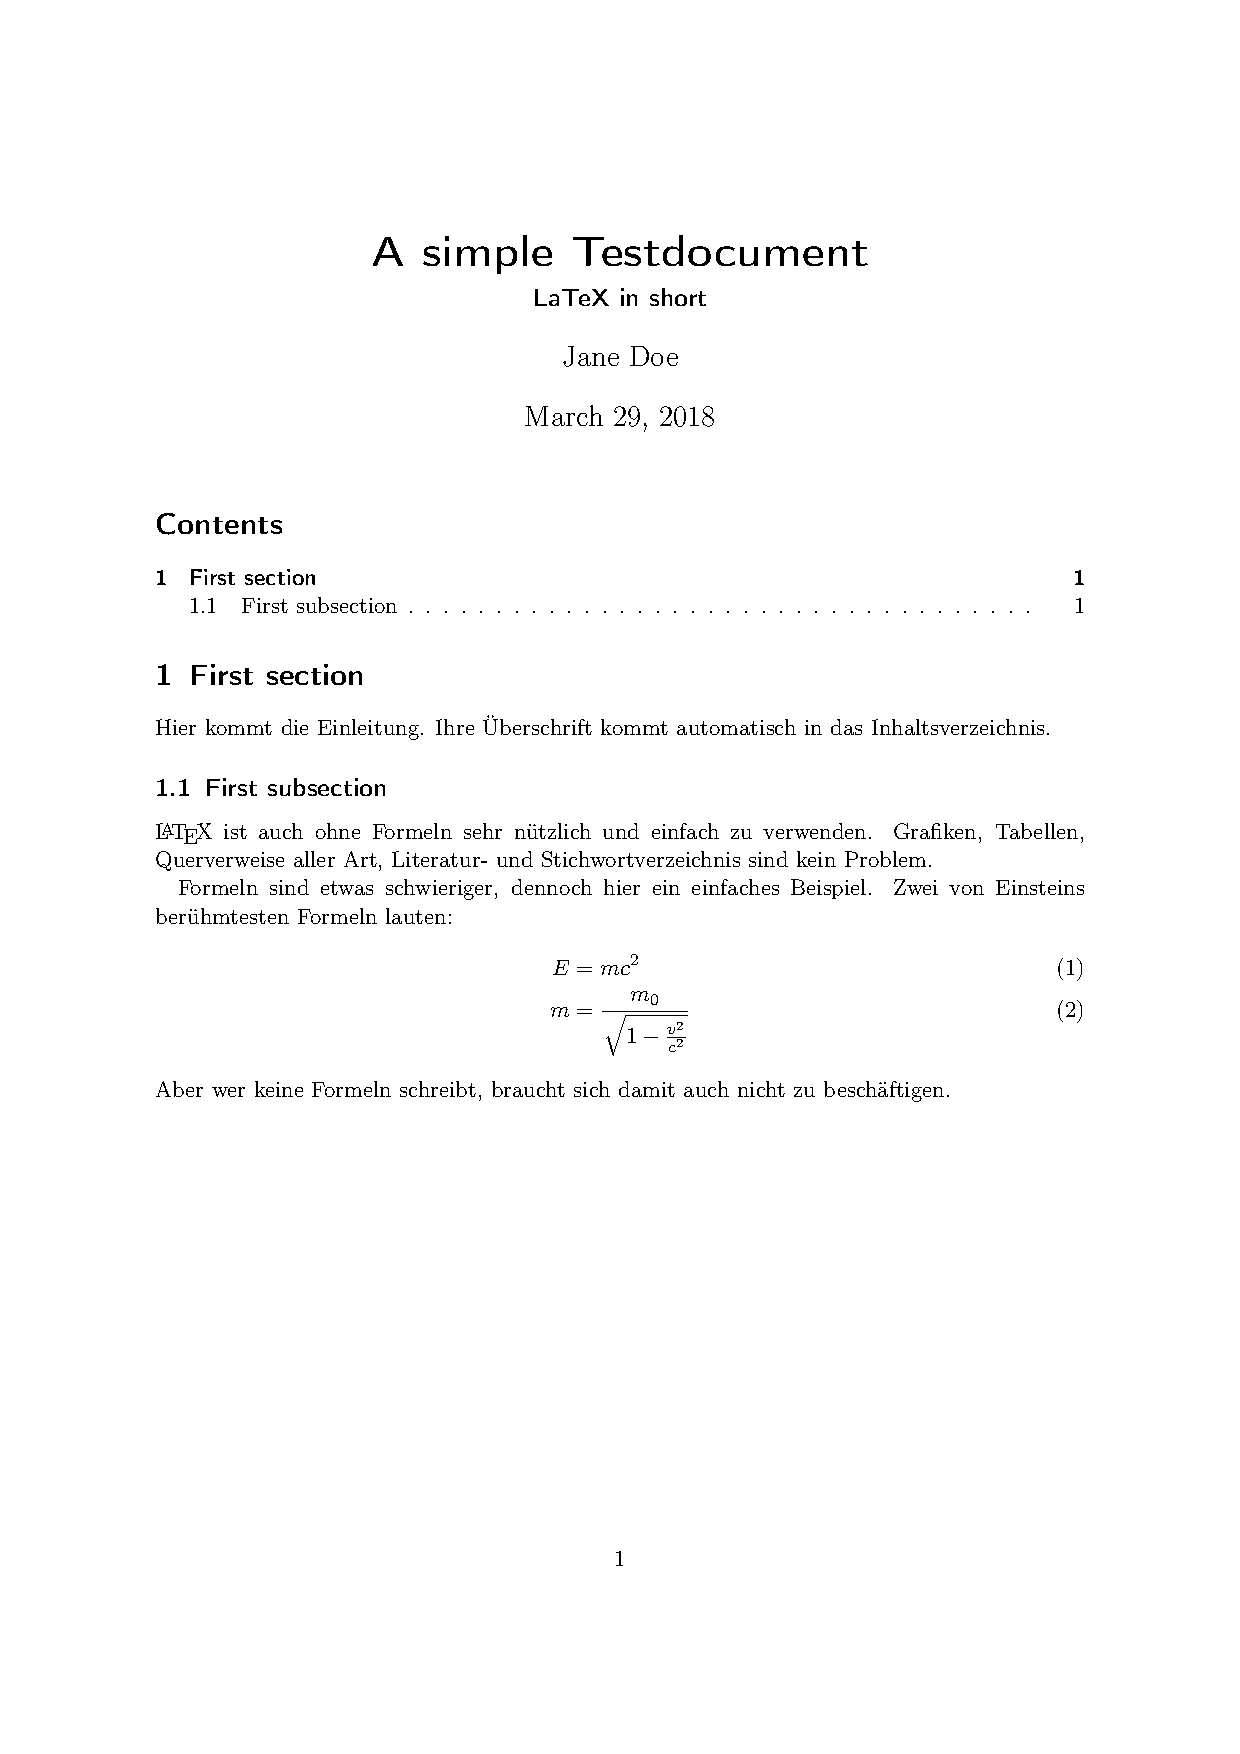
\includegraphics[width=\textwidth]{example}}
%\end{minipage}
\end{document}
